\section{Formalizing the Mutable Data Plane}
\label{sec:formal}
The previous sections argued why a new approach to network verification is needed and briefly outlined what it might look like.
In this section, we sketch a concrete way to formalize and prove interesting  properties of networks of middleboxes.

\begin{lstlisting}[caption={Model for an IDS},label=list:ids,captionpos=t,float,abovecaptionskip=-\medskipamount,
                    numbers=left,
                    morekeywords={oracle, model, when, default, state, forward},belowskip=-0.1in]
oracle suspicious? (packet: Packet) : Boolean;

model ids (p: Packet) = {
  when suspicious?(p) =>
      forward {}
  default =>
      forward {p}
}
\end{lstlisting}

% \subsection{Verification Problem}
DeMillo et al.~\cite{popl:DeMilloLP77} previously argued that specifying the desired behavior of a program (or network) is hard. 
Indeed, the lack of a precise specification is a major problem for program and network verification. 

The primary function of networks is to allow hosts to communicate with each other. Reachabality, the property that a certain class of packets sent from host $A$ can reach host $B$, and its converse, isolation, are fundamental to networks: all useful networks must satisfy some set of reachability properties and their verification is thus universally important. In the rest of this section we limit our discussion to Reachability invariants.

We formally state these invariants using temporal logic where we assume fairness, \ie we assume any continuously enabled transition will eventually occur. 
First, we define two relations: $Send(n, p)$ indicating some network entity (node) $n$ sent
a packet $p$ (at some time), and $Recv(n, p)$ indicating node $n$ received packet $p$. Given these relations any reachability property can be expressed in
LTL (Linear Temporal Logic) as
\begin{align*}
\forall p\in \text{Packet}: \Box (Send(src, p) \land Predicate(p) \implies \Diamond(Recv(dest, p)))
\end{align*}
This temporal logic statement says that a packet $p$ sent by $src$ which satisfies $Predicate$ is eventually received by $dest$.
Similarly, isolation can be formally expressed by requiring that a packet sent by $src$, satisfying $Predicate$ is never received by $dest$:
\begin{align*}
\forall p\in \text{Packet}: \Box (Send(src, p) \land Predicate(p) \implies \Box(\neg Recv(dest, p)))
\end{align*}

$Predicate$ in the definitions above is specified using the same abstractions used to specify network policies, \ie either in terms of packet
header fields (source, destination, etc.) or in terms of the abstraction provided by a middlebox oracle (\S\ref{sec:mbmodel}). For example, a property
saying no SSH traffic can reach a server $d$ can be expressed as
\begin{align}
\forall s\in \text{Node}, p\in \text{Packet}: \Box (Send(s, p) \land ssh(p) \implies \Box(\neg Recv(d, p))) \label{eq:isossh}
\end{align}

where $ssh(p)$ returns true if an Oracle classifies the packet as belonging to an SSH connection.
We reason about reachability and isolation properties assuming that the Oracles are correct.
Verifying the isolation property in Equation~(\ref{eq:isossh}) therefore requires answering the question:
``assuming SSH traffic is correctly identified, can a packet belonging to an SSH connection reach $d$?''

% \subsection{Formalizing Middlebox Semantics}

% \notepanda{I think we should cut this bit, or move it elsewhere}
As stated earlier, we model a middlebox as an oracle and a simple abstract model. The Oracle provides abstractions that are used to specify the
properties being checked. We expect models for middleboxes (which include both an oracle and a generic model) to be specified
using a constrained programming language. Listing~\ref{list:ids} shows an example of such a specification
for an intrusion detection system (IDS). The IDS oracle provides one abstraction, \texttt{suspicious?}, defined in the first line. The abstract model is
defined in Lines 4 -- 9 and uses this abstraction. First we check to see if the packet is suspicious (the Oracle's decision here might be based on what
packets it has seen previously), and  drop the packet (Line 6) or forward the packet (Line 9) depending on the value returned by the Oracle.
% \notepanda{End of where we would cut until}

Next, we develop abstract semantics for middleboxes. We use these to reason about general properties (such as composition) that apply to all middleboxes. Our semantic model is defined over a potentially infinite set of packets, $P$.  We augment packets to include information about their location (\ie the
middlebox or
switch port). We also define the operator $\doteq$, such that $p_1 \doteq p_2$ implies that packets $p_1$ and $p_2$ are identical except for their location.
Finally, we use $P^*$ to represent the set of all (potentially unbounded) sequence of packets.
The abstract model middlebox $m$ is a function $m\colon P\times P^* \to 2^P$ which takes a packet ($p\in P$) and a history ($h\in P^*$) 
of all the packets that have
previously been processed by $m$ and produces a (possibly empty) set of packets $m(p, h)$. Given this model a switch is a simple function for which
$m(p, h) \doteq \left\{p\right\}$. Similarly a simple firewall, $f$ (whose decision process is represented by $allowed$) can be expressed as
\begin{align*}
 f(p, h) = \begin{cases}
    \left\{p'\right\}\ p' \doteq p & \mbox{if } allowed(p, h)\\
    \left\{\right\} & otherwise
 \end{cases}
\end{align*}

% \subsection{Composing Middleboxes}
Ideally, we would like to be able to reason about the network \emph{compositionally}, \ie the correctness of the network should follow from
the correctness of smaller, simpler components. Compositional reasoning can reduce the cost of verification and enable incremental verification
of changes in the network. Compositionality also allows us to potentially verify invariants in much larger networks, both by allowing us to parallelize verification and by reducing the size of the problem that needs to be provided to the SMT solver. Compositionality has been important for making verification tractable in other domains, for instance the use of rely-guarantees~\cite{tse:MisraC81,ifip:Jones83}, was important for enabling verification of concurrent programs.

% \cbstart
We start by defining what it means to be able to compositionally verify a network. Let us define the union of two networks $N_1$ and $N_2$ in the natural way, \ie $N_1\cup N_2$ contains the union of all nodes and links in each of $N_1$ and $N_2$. Consider two networks: $N_1$, where property $P_1$ holds (represented as $N_1\models P_1$); and $N_2$, where property $P_2$ holds. We can compose the proofs for properties $P_1$ and $P_2$ if and only if  both $P_1$ and $P_2$ hold for $N_1 \cup N_2$. For example, consider verifying the invariant ``$A$ and $B$ cannot receive data from $S$'' in network $N$ in Figure~\ref{fig:compose_fail}. If compositional verification is possible for $N$, then the property holds in $N$ if and only if $A$ cannot receive data from $S$ in $N_1$, and $B$ cannot receive data from $S$ in $N_2$. More formally, we can verify properties $P_1$ and $P_2$ compositionally for network $N$ if for any $N_1 \subset N$ and $N_2\subset N$
\begin{align*}
N_1 \models P_1,  N_2\models P_2\\
\hline
(N_1 \cup N_2) \models P_1\land P_2
\end{align*}
% \cbend


\begin{figure}[t]
\centering
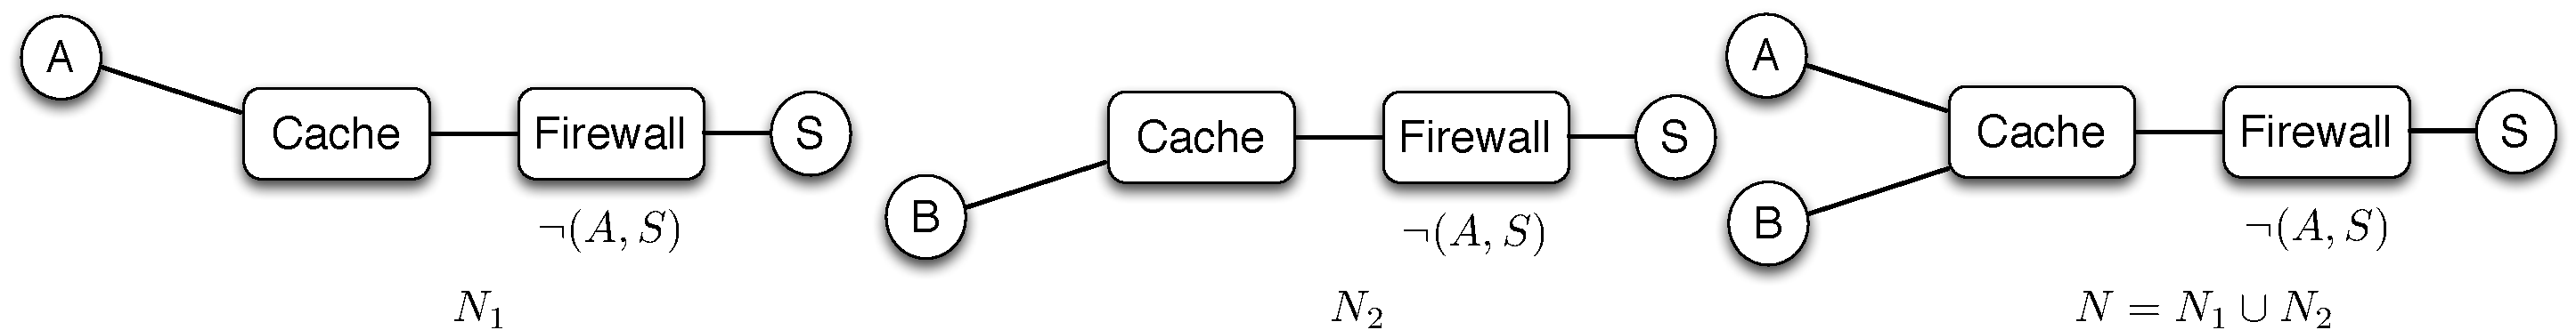
\includegraphics[width=0.9\textwidth]{figures/rono_example.pdf}
\caption{Example where networks are not composable with respect to reachability properties.}
\label{fig:compose_fail}
\vspace{-0.15in}
\end{figure}

Generally, one cannot perform compositional verification of reachability properties. For instance,
consider the example in Figure~\ref{fig:compose_fail}. The cache in this example records all requests to and the corresponding responses from $S$.
On receiving a new request,  the cache checks to see if it has previously recorded a response for this request, in which case it returns the saved response;
otherwise the cached forwards the request, unmodified, to the firewall. The firewall drops all requests sent from $A$ to $S$, but otherwise forwards all other requests and responses unmodified. In network $N_1$, $A$ can never receive a response from $S$ (thus is isolated). However in the composed network $N_1\cup N_2$, if $B$ sends a request $r$ and receives response $r'$ from $S$, then $A$ can also request $r$ and receive $r'$.

One key insight is that despite being impossible in general, there exists an important subset of networks where compositional reasoning can be used
to verify reachability properties. We have found that networks which contain only a special class of middleboxes, Rest-of-Network Oblivious (RONO) middleboxes (\S\ref{sec:modelnet}) are often amenable to compositional verification. A RONO middlebox is one whose forwarding behavior (which is all we care about for reachability and isolation) for a pair of hosts depends only on the traffic sent between these hosts. More formally, define the restriction $h|_{(A, B)}$ of a packet history $h\in P^*$  to be the largest subsequence of $h$ containing only those packets that were sent between host $A$ and $B$; we then define a middlebox $m$ to be RONO if and only if
\begin{align*}
\forall p: p.src = A \land p.dest = B &\ \  f(p, h) = f(p, h|_{(A, B)}) \text{   and}\\
\forall p: p.src = B \land p.dest = A &\ \ f(p, h) = f(p, h|_{(A, B)}) \numberthis \label{eq:rono}
\end{align*}
Similarly, we define an entire network as RONO, if its semantics can be described using a function that meets the condition stated in Equation~\ref{eq:rono}.

\begin{figure*}[t]
\centering
\subfloat[]{
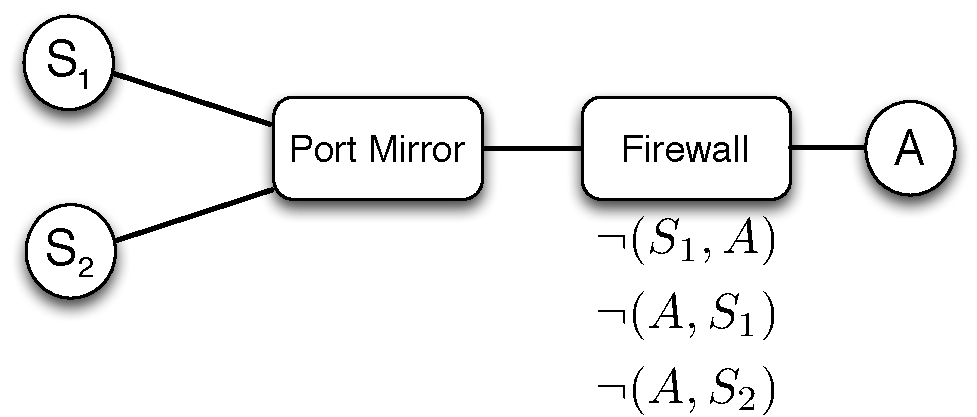
\includegraphics[width=0.3\textwidth]{figures/rono_composition_bad.pdf}
\label{fig:rono_all}
}
\subfloat[]{
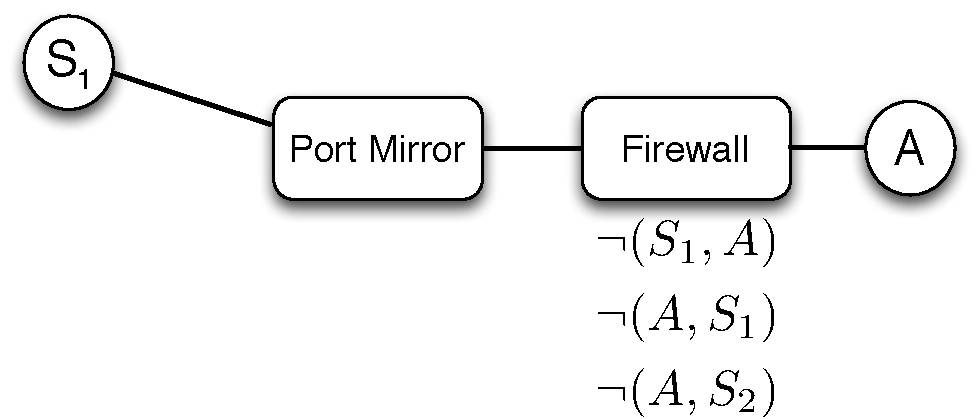
\includegraphics[width=0.3\textwidth]{figures/rono_composition_bad_a.pdf}
\label{fig:rono_a}
}
\subfloat[]{
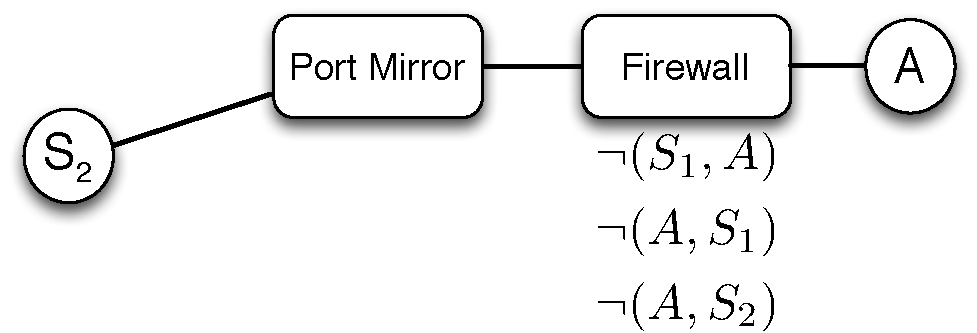
\includegraphics[width=0.3\textwidth]{figures/rono_composition_bad_b.pdf}
\label{fig:rono_b}
}

\caption{Example where the composition of two RONO middleboxes is not RONO.}
\label{fig:rono_fail}
\vspace{-0.15in}
\end{figure*}

Surprisingly, we find that not all networks that contain only RONO middleboxes are RONO, \ie RONO is not closed under composition. For example, consider the network in Figure~\ref{fig:rono_fail}. The firewall in this example is stateful and is configured to allow \emph{no communication} between $A$ and $S_1$. Furthermore, the firewall configuration allow $A$ and $S_2$ to communicate, provided $A$ establishes the connection, \ie sends the first packet. The port mirror is configured to duplicate and send all packets received from the firewall to both $S_1$ and $S_2$. Beyond these policies, both the firewall and port mirror forward traffic as expected (\ie they forward packets towards their intended destination). In this example, the port mirror is stateless, and hence trivially RONO according to Equation~\ref{eq:rono}. The behavior of the stateful firewall is also RONO. However, the composition of these two middleboxes is not RONO. When we consider just $S_1$ and $A$ in isolation (Figure~\ref{fig:rono_a}), \ie a case where $S_2$ neither sends nor receives any packets, $A$ and $S_1$ cannot communicate, since all packets between them are dropped at the firewall. However, when we remove this restriction, \ie allow $S_2$ to send or receive packets, we find that $A$ can in fact communicate with $S_1$: $S_2$ needs to first send a packet establishing a connection with $A$, any subsequent responses sent by $A$ are allowed through the firewall, and duplicated so they are received by both $S_1$ and $S_2$. Therefore, it is simple to see that the abstract semantics of the network are different depending on whether we consider the entire packet history or a restriction, and the network is therefore not RONO, despite containing only RONO middleboxes. This shows that RONO is not closed under composition, \ie the composition of two RONO middleboxes might not be RONO. 

However, despite RONO not being closed under composition in general, we have found that many existing networks are in fact RONO, and are hence amenable to compositional verification. Further, given that operators frequently add new middleboxes to their network, and RONO networks are precisely those where such addition cannot disrupt unaffected parts of the network, we think that many existing network might, in fact, be RONO by design.